\documentclass[12pt]{article}

\usepackage{sbc-template}

\usepackage{graphicx,url}

%\usepackage[brazil]{babel}   

\usepackage[utf8]{inputenc}  

\usepackage{hyperref}

\newcommand\tab[1][1cm]{\hspace*{#1}}

\sloppy

\title{Classificação de flores utilizando Redes\\ Neurais Convolucionais}

\author{Walter H. Silva\\\href{walter.silva@ufv.br}{walter.silva@ufv.br}}

\address{Universidade Federal de Viçosa - Campus Rio Paranaíba\\
  Minas Gerais, BR
}

\begin{document} 

\maketitle

\begin{abstract} 
  This work aims the implementation and analysis of Deep Learning models for the classification of flowers of 102 different species. Classification is a type of learning, which aims to better approximate functions that represent the linear or non-linear separation of data. In this context, the classification of flowers is interesting for several areas such as biology, botany, medicine, etc. Convolutional Neural Networks are a category of algorithms in the Deep Learning field, which proved to be excellent algorithms as opposed to the classical Machine Learning methods, generating an accuracy of 97\% in flower classification.
\end{abstract}

\begin{resumo} 
  Este trabalho visa a implementação e análise de modelos de Aprendizagem Profunda para a classificação de flores de 102 espécies diferentes. Classificação é um tipo de aprendizagem, que visa melhor aproximar funções que representem a separação linear ou não linear de dados. Neste contexto, a classificação de flores se mostra interessante para diversas áreas como a biologia, botânica, medicina, etc. Redes Neurais Convolucionais são uma categoria de algoritmos do campo de Aprendizagem Profunda, que se mostraram excelentes algoritmos em contraposição aos métodos clássicos de Aprendizagem de Máquina, gerando uma acurácia de 97\% na classificação de flores.
\end{resumo}

\section{Introdução}

\tab\tab[0.5pt] Iris \cite{Iris} é um conjunto de dados de flores lançado em 1936, que possui 4 atributos referentes as características de 3 espécies flores. Em razão de sua simplicidade o conjunto é utilizado como exemplo para o ensino em áreas como o Aprendizado de Máquina, Aprendizagem Profunda, Mineração de Dados, etc. O conjunto de dados de flores de 102 espécies \cite{Flower} tem o intuito de desafiar os modelos de Aprendizagem Profunda contemporâneos, uma vez que o mesmo possui 102 espécies e sua complexidade se eleva consideravelmente se comparado ao conjunto Iris.
	
O desafio em questão é proposto como projeto final do curso online da Udacity e do curso presencial de Aprendizagem Profunda da Universidade Federal de Viçosa - Campus Rio Paranaíba. Diferentes arquiteturas de Redes Neurais Convolucionais, assim como seus hiperparâmetros serão abordados a fim de obter uma melhor acurácia na separação das espécies de flores e por conseguinte auxiliar na tarefa de classificação realizada por humanos, que se encontra a merce do viés ou erro humano. A utilização de Redes Neurais Convolucionais se faz presente em razão da excelente capacidade das mesmas em lidar com a extração de características, onde a relação entre as variáveis é complexa.

\section{Configuração dos Experimentos}

\subsection{Conjunto de dados}

\subsubsection{Treinamento}

\tab\tab[0.5pt] O conjunto de dados de flores de 102 espécies \cite{Flower} foi utilizado como treinamento. Por se tratar de um problema de classificação, as classes atribuídas ao conjunto de dados em questão foram utilizadas. O conjunto de treinamento se consiste em 102 espécies diferentes de flores, cada uma contendo de 40 a 248 imagens RGB de largura 400-700 pixels e altura 500 pixels, total de 6552 imagens.

As imagens em questão foram redimensionadas, transformadas para tensores e normalizadas, além disso o aumento de dados foi aplicado, gerando  5 novos conjuntos de dados:

\begin{enumerate}
    \item Conjunto 2: imagens rotacionadas entre -30º e 30º
    
    \item Conjunto 3: imagens transformadas  para brilho 0-100\%, hue 50\% e saturação 50\%
    
    \item Conjunto 4: imagens recortadas randomicamente, largura 224 pixels e altura 224 pixels
    
    \item Conjunto 5: imagens invertidas horizontalmente
    
    \item Conjunto 6: imagens invertidas verticalmente
\end{enumerate}

Após o aumento de dados a quantidade total de imagens é de 39,312 mil imagens. A figura 1 ilustra parte do conjunto de treinamento.

\begin{figure}[ht]
\centering
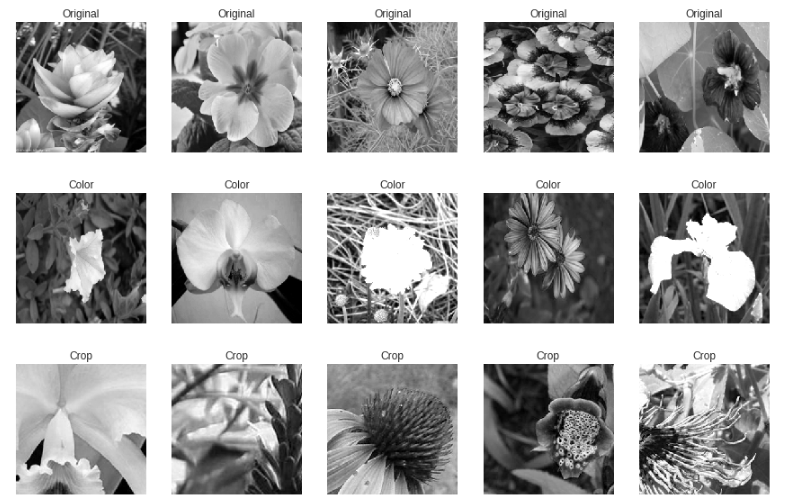
\includegraphics[width=.9\textwidth]{train.png}
\caption{Treino}
\label{fig:train}
\end{figure}

\subsubsection{Validação}

\tab\tab[0.5pt] O conjunto de validação se consiste de 818 imagens, diferentes das imagens de treinamento não geradas artificialmente, representando 102 espécies diferentes de flores. Ĩmagens RGB de largura 400-800 pixels e 500-800 pixels de altura. As imagens de validação foram redimensionadas, transformadas para tensores e normalizadas. A figura 2 ilustra parte do conjunto de validação.

\begin{figure}[ht]
\centering
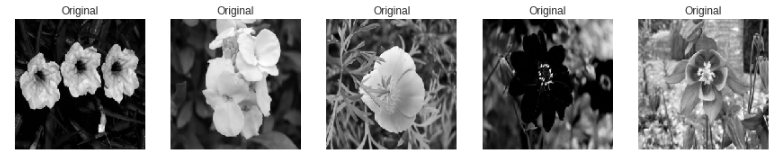
\includegraphics[width=.9\textwidth]{valid.png}
\caption{Validação}
\label{fig:valid}
\end{figure}

\subsubsection{Testes}

\tab\tab[0.5pt] As imagens de testes são 20\% das imagen de validação, contudo neste trabalho as mesmas não foram utilizadas, ou seja, o conjunto de validação não foi alterado.

\subsection{Ferramentas}

\tab\tab[0.5pt] PyTorh é um framework criado por engenheiros do Facebook com o intuito de facilitar a criação de modelos de alto nível utilizando arquiteturas consideradas o estado da arte, além de ser modularizado e extremamente rápido, possuindo uma API escrita em C++ e ONNX, utilizada para a exportação dos modelos. Alternativas como o framework Keras e Sonet foram consideradas, contudo PyTorch se mostrou uma melhor opção em ambas as características mencionadas do mesmo.

Os experimentos foram executados através de uma GPU Tesla K80 e uma GTX Mx 150, utilizando-se da tecnologia CUDA.

\subsection{Arquiteturas}

\subsubsection{ResNet 18}

\tab\tab[0.5pt] ResNet 18 \cite{Resnet18} é uma arquitetura de Rede Neural Convolucional de 18 camadas, que evita o desaparecimento do gradiente, isso é realizado através da adição da entrada da camada anterior a saída da camada atual, a figura 3 ilustra o processo descrito. A arquitetura em questão foi configurada para utilizar o aprendizado do treino do conjunto de dados Image Net, assim como as duas primeiras camadas da Rede Neural foram congeladas.

\begin{figure}[ht]
\centering
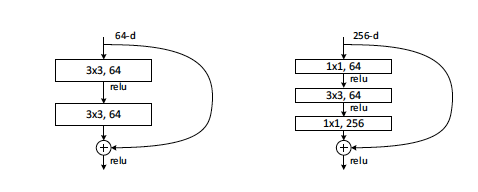
\includegraphics[width=.9\textwidth]{resnet18.png}
\caption{ResNet 18 - Arquitetura}
\label{fig:resnet18}
\end{figure}

\subsubsection{VGG 11}

\tab\tab[0.5pt] VGG 11  \cite{Vgg11} é uma arquitetura de Rede Neural Convolucional de 11 camadas, que diminui o custo computacional através da definição de filtros convolucionais com tamanho específico durante toda a Rede Neural, a figura 4 ilustra a arquitetura descrita. A arquitetura em questão foi configurada para utilizar o aprendizado do treino do conjunto de dados Image Net, assim como o primeiro bloco de convolução foi congelado.

\begin{figure}[ht]
\centering
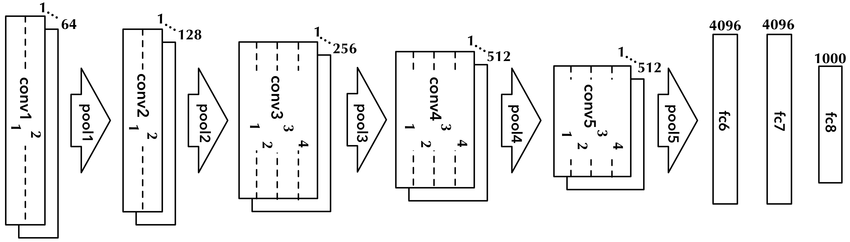
\includegraphics[width=.9\textwidth]{vgg11.png}
\caption{VGG 11 - Arquitetura}
\label{fig:vgg11}
\end{figure}

\section{Resultados e discussões}

\subsection{ResNet 18}

\tab\tab[0.5pt] A Rede Neural Convolucional ResNet 18 foi inicialmente treinada com batchs de tamanho 124, optimizador SGD com taxa de aprendizado de 0.001 e todos os conjuntos de dados, obtendo 87\% de acurácia, contudo em razão dos altos valores nos híper parâmetros mencionados, a rede não performa como esperado. Ao reduzir o tamanho dos batchs para 12, optimizador ADAM, que se adapta ao longo da propagação da rede, com taxa de aprendizado de 0.0001 e todos os conjuntos de dados, a taxa de acurácia foi de 97\%, assim como a figura 5 ilustra.

\begin{figure}[ht]
\centering
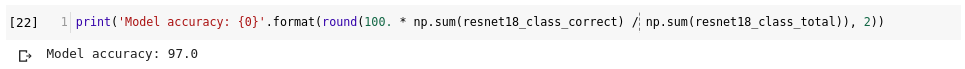
\includegraphics[width=.9\textwidth]{resnet18_accuracy.png}
\caption{ResNet 18 - Acurácia}
\label{fig:resnet18accuracy}
\end{figure}

\tab\tab[0.5pt] Decrementar os hiperparâmetros mencionados causa uma taxa de aprendizado lenta, contudo concisa, que evita o desaparecimento do gradiente, ou seja, o gradiente não para na local mínima.

\tab\tab[0.5pt] O gráfico da perda do treinamento ilustra picos, que são ocasionados em razão da entrada de um novo conjunto de dados na fase de treinamento, isso se trata de uma hipótese, que pode ser confirmada randomizando todos os conjuntos de treinamento.

\tab\tab[0.5pt] Nenhuma semente foi definida, contudo o modelo foi treinado múltiplas vezes para garantir o resultado de 97\% de acurácia obtido, treinado com múltiplas combinações de hiperparâmtros e conjuntos e ordem dos conjuntos de treinamento, assim como o treinamento foi salvo e encontra-se disponível no repositório do Github \cite{Sphinxs}.

\begin{figure}[ht]
\centering
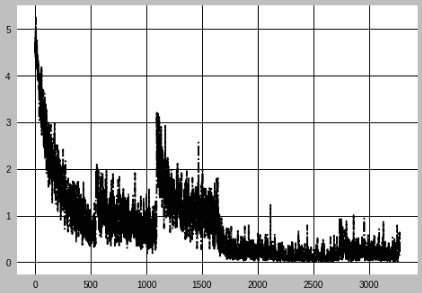
\includegraphics[width=.9\textwidth]{resnet18_loss.png}
\caption{ResNet 18 - Perda}
\label{fig:resnet18loss}
\end{figure}

\subsection{VGG 11}

\tab\tab[0.5pt] A partir do aprendizado de como treinar um modelo, obtido no treinamento da rede ResNet 18, o treinamento da rede VGG 11 se deu inicialmente através de batchs de tamanho 12, optimizador ADAM com taxa de aprendizado de 0.0001 e todos os conjuntos de dados, obtendo 87\% de acurácia, contudo neste caso apenas o tamanho de batch se fez um bom parâmetro, uma vez que tal rede requer um poder computacional vezes maior do que a rede ResNet 18. Para a melhoria do modelo foi aplicado o optimzador SGD com taxa de aprendizado de 0.001 e batchs de tamanho 12, obtendo 92\% de acurácia, assim como a figura 7 ilustra.

\begin{figure}[ht]
\centering
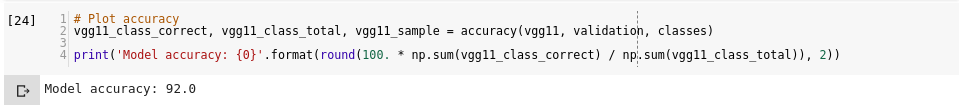
\includegraphics[width=.9\textwidth]{vgg11_accuracy.png}
\caption{VGG 11 - Acurácia}
\label{fig:vgg11accuracy}
\end{figure}

\tab\tab[0.5pt] Uma taxa de aprendizado maior demonstra-se interessante para a arquitetura VGG 11, por mais que a mesma não possa ser intuitiva, uma vez que pode ocasionar o desaparecimento do gradiente, ou seja a parada ou loop na local mínima.

\tab\tab[0.5pt] A mesma característica referente ao treinamento com múltiplos conjuntos de dados se fazem presente no treinamento da rede VGG 11, como é ilustrado na figura 8.

\begin{figure}[ht]
\centering
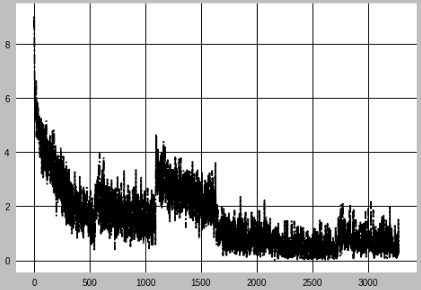
\includegraphics[width=.9\textwidth]{vgg11_loss.png}
\caption{VGG 11 - Perda}
\label{fig:vgg11loss}
\end{figure}

\section{Conclusão}

\tab\tab[0.5pt] Conclui-se que o processamento e escolha de arquitetura, assim como a configuração de seus hiper parâmetros, causam um grande impacto no resultado final. Nete trabalho o aumento de dados, uma baixa taxa de aprendizado e batchs pequenos ocasionaram um melhor resultado, contudo tais aspectos também ocasionam um grande custo computacional.

Buscar um abordagem de meta aprendizado, aprendizagem por reforço, aprendizagem não supervisionada, etc; pode ser estudado em trabalhos futuros, assim como a utilização de K-Fold, Synthetic Data, randomização dos dados de treinamento, etc.

\bibliographystyle{sbc}

\bibliography{sbc-template}

\end{document}